\chapter{Related Work}
\label{cha:literature}

In this chapter we will go through a number of existing solutions. First we discuss some well known
HPC products which offer a complete set of features to launch and operate an HPC site. These are
mostly large scale software which include every aspect of data intensive computing. 
Then we introduce data distribution solutions which are designed to manage big data. Afterwards
we introduce some state distribution solutions which could be utilized in a possible solution to
spread object states among a number of programs. At the end we introduce some existing efforts
in scientific workflow management field. At each part we introduce a the parameters which are
interesting for us and then we analyze the given product against them.

It is also important to mention that we have only considered mostly free and open source projects. 
Projects which need royalty fees or limit the use cases and their code is not available
publicly have not been considered. Rationale for this decision is to achieve a 
sustainable solution for small groups with limited budgets. Therefore it is crucial to avoid
any notable costs in relation with using products and implementing non-free and non-open standards or protocols.
In case of closed source programs it would not be possible to extend them and in case of protocols it is
obviously a bad choice because it will impose future risks on us. 
Therefore we decide to avoid such products, standards or protocols all together.


\section{Grid Computing Solutions}
There are various products in high performance computing field, such as grid middlewares, distributed
storage systems, data storage management systems, workflow managers, operating systems for massively parallel 
super computers and so on. Most of these products are targeted toward super computers and large scale
operations. However we require more light weight solution toward small, distributed groups. 
Therefore in this section we do not want to go through
all the existing products in HPC field, which is out of scope, instead we discuss a number of them
which are more likely to be used in European scientific communities, specially in the working 
environment that I am accomplishing my work.

It is importance to notice that we asses these products against 
requirements of small and agile scientific groups which often only have access to limited resources.
Moreover we look for an application level solutions and not a sole product.
Here are the extracted parameters according to the discussed requirements:

\begin{itemize}
\item Deployment complexity
\item Data provision methods
\item State preservation
\item Centralization
\item Required user rights
\item Runtime control
\item Applicability
\end{itemize}
Here go through a number of projects which are widely being used.
\subsection{UNICORE}
UNICORE is one of the main providers of European Middleware Inititative(EMI) \cite{EMI}. 
It is an open source software under BSD license\footnote{\url{https://www.unicore.eu/unicore/}}.
It follows a client/server architecture and is implemented in Java programming
language.
In consists of three main layers, user, server and target system layer. 
Jobs will be executed from the client machine and the resulting output files will be downloaded
to the same machine as well. It provides job execution and monitoring on grids.\cite{unicore_wp}

It has a graphical client based on Eclipse IDE. There
is also a command line interface available. GUI provides workflow design and execution means and 
allows users to design complex workflows and combine multiple applications while selecting
the desired amount of RAM and number of CPUs on target resources. It introduces a concept 
called GridBeans that allows users to extend the GUI to take advantage of software available on
the grids and visualizing output data.

The service layer of UNICORE is composed of Gateway and number of other components. Gateway, as
its name says, is the entry point to a UNICORE site. It is like the middle-man between inside
and outside world in UNICORE. Client makes job specification in Job Service Description Language
 (JSDL)\footnote{\url{http://en.wikipedia.org/wiki/Job_Submission_Description_Language}}.
 This layer exposes resources via Web Services Resource Framework (WSRF) compliant web 
 services\footnote{\url{http://en.wikipedia.org/wiki/Web_Services_Resource_Framework}}
 for file transfer, job submission and management. There are also a wide range of file transfer
 protocols supported for site-to-site and 
 client-to-site\footnote{\url{https://www.unicore.eu/unicore/architecture/service-layer.php}}.

It has been used in super-computing domain to allow exposing and managing of available 
computing resources.\cite{unicore_arch}

\subsubsection {Deployment complexity}
Deployment requires Java Runtime Environment in place, which if not available would require 
further assistance from IT administrators to be installed. It is also intended to be installed
on a cluster site not normal workstations. To access web features a browser plugin should be
installed\footnote{
\url{https://www.unicore.eu/documentation/manuals/unicore/files/client_intro.pdf}}.
The server is composed of multiple components that user 
has to download and install each of them separately.
\subsubsection {Required user rights}
To install the server components admin rights on Windows or root access on Unix-like operating
systems are necessary. Even though running the client does not need any special permissions.
\subsubsection{Data provision methods}
Output files are produced on remote resource (service layer) and can be downloaded to client
machine on demand. Input files should be transferred to the UNICORE storage using the client.
There are also command line tools such as \textit{uftp} to transfer files to remote 
storages\footnote{
\url{https://www.unicore.eu/documentation/manuals/unicore/files/uftpclient/uftpclient-manual.pdf}}.
UNICORE relies on standard file system as storage mechanism. However there are efforts to 
extend it to support Hadoop Distributed File System as a storage mean.\cite{wasim2009}
\subsubsection {State preservation}
The UNICORE service layer contains the state of the application and running jobs. 
Upon connecting to a UNICORE site users can utilize the GUI to explore 
the site and access the running jobs for control and monitoring purposes.
The details of possible operations are covered in UNICORE user manuals.

\subsubsection {Centralization}
UNICORE follows a standard client-server architecture therefore it is centralized. It sits on 
top of a cluster and will let clients to connect to it via defined services. There is no means
of inter-site and inter-unicore information exchange. UNICORE is a grid middleware and
infrastructure and therefore it is not intended for inter-site state distribution.
\subsubsection {Runtime control}
It is possible to use UNICORE's web services from third party applications, however this does 
not give control over the run-time internals of the application, instead it is merely a way 
to write extensions for the program.
\subsubsection {Applicability}
There are a number of considerations that prevent us from taking UNICORE as a solution. However
it is a well established and mature product on its own.

UNICORE is supposed to be a site manager software. A group have to install it on a cluster and
then users will be able to access the resources. Only a well-informed and skilled group can 
install and maintain such a product, which contradicts with our initial requirement that is 
aimed toward small groups. Moreover we look for a user space solution which is not the case
about UNICORE.

Then next point is distribution of data and state. Even though the product which is installed
on a site will preserve state of jobs and will alow accessing remote file systems, still it is
not a good fit for our case. We need to have automatic inter-site interoperability, both for
data distribution and state of the system, i.e. running jobs, which is not fulfilled by this
product.

Runtime control over a job execution is another limitation that we face with this solution.
We need to be able to deliberately interfere in every step of execution of a job and define 
arbitrary policies for them. To fulfill this, we more need a framework rather than an application.
Applications such as UNICORE represent computing backends and job schedulers rather than a 
platfrom to build new solutions on top of them.

\subsection{Globus Toolkit}
Globus Toolkit (GT) is the widely developed application for resource management and grid computing today.\cite{eickermann2005steering}
It lets people share resources, such as computational power, databases, etc online while preserving the
provider's local autonomy. It consists of various modules and allows further services
to use GT libraries to build new services.\cite{foster2005network}

Unlike UNICORE which is heavily dependent on its Eclipse based client, 
GT does not provide an interactive user interface. However it offers its services in form of multiple command 
line tools that makes them suitable to be used in 
scripting\footnote{\url{http://toolkit.globus.org/toolkit/docs/4.0/data/key/}}.

\subsubsection {Deployment complexity}
GT has various components that the user might not need all of them and should install whatever she is
interested in. Services only install on Unix-like operating systems. Providing a Unix-like environment
such as \textit{cygwin} one can install it under Windows as well. It is also possible to install it directly
from pre-compiled binaries or install from source, since GT is free software and is available mainly
under Globus Toolkit Public License (GTPL)\footnote{\url{http://toolkit.globus.org/toolkit/docs/6.0/licenses/}}.

\subsubsection{Data provision methods}
GT implements GridFTP protocol\footnote{\url{https://www.ogf.org/documents/GFD.20.pdf}} as defined by Open Grid Forum (OGF).
Users have to use command line tool as well as some GUIs provided by GT to move files between local and remote 
machines before and after executing jobs.
\subsubsection {State preservation}
GT has a component called Grid Resource Allocation and Management (GRAM) which provides job submission, management
and monitoring. GRAM is not a Local Resource Manager (LRM)\footnote{Local job managers control a resource
directly and let the jobs to be executed on them, e.g. Sun Grid Engine (SGE), Condor, etc.}, instead it utilizes
them to execute jobs on remote sites. 
GT supports WSRF specification, therefore it has statefull web services, however there is no notion of inter-side workflow
and state preservation.
\subsubsection {Centralization}
GT could be installed on multiple machines to allow users to run GT services on them. These machines will communicate
based on X.509 security standard. Having multiple machines, Globus Gatekeeper will dispatch services on them allowing
GRAM to submit jobs onto whatever LRM available.
\subsubsection {Required user rights}
User should have admin rights to install and configure Globus Toolkit along with its components.
\subsubsection {Runtime control}
Even though GT allows very flexible scripting and lets to develop services using its libraries, there is no notion
of full runtime control rather than predefined routines such 
as MPI\footnote{http://toolkit.globus.org/alliance/publications/papers/gempi.pdf}.
\subsubsection {Applicability}
Like UNICORE, GT is a product rather than a framework to build new services on top of it. However it is more flexible
in terms of developing new services on top of it. It could be utilized as another backend to our solution which makes it
possible to take advantage of a wide range of HPC resources in our solution. But itself alone is not sufficient for 
our mission.

\section{Distributing Data}
%Before introducing approaches toward data distribution we define our parameters:
%\begin{itemize}
%\item Deployment complexity
%\item Data provision methods
%\item State preservation
%\item Centralization
%\item Required user rights
%\item Runtime control
%\item Applicability
%\end{itemize}

\subsection{Distributed File Systems}
One way to achieve fault tolerant and reliable data storage and access is to use
distributed file systems (DFS). In this case the data will be replicated over a
network of storage servers with different magnitudes based on the underlying file
system. We will discuss a number of free and open source solutions.

\subsubsection{Hadoop Distributed File System (HDFS)}
Here we discuss HDFS and not Hadoop itself, but here is a short description of what Hadoop is:
``Apache Hadoop is a set of algorithms (an open-source software framework written in Java) 
for distributed storage and distributed processing of very large data sets (Big Data) 
on computer clusters built from commodity hardware\footnote{\url{http://en.wikipedia.org/wiki/Apache_Hadoop}}.''
Thus it targets the same goals that we have but in very large scale with a different approach.
``The Hadoop Distributed File System (HDFS) is a distributed file system designed to run on
commodity hardware.'' 
The primary objective of HDFS is to store data reliably even in the presence of failures.\cite[tp.~3]{HDFSDocuments}

``Hadoop1 provides a distributed file system and a framework 
for the analysis and transformation of very large data sets 
using the MapReduce \cite{DG04} paradigm.''\cite{TheHDFS}

``HDFS stores metadata on a
dedicated server, called the NameNode. Application data are stored on
other servers called DataNodes.''\cite{TheHDFS}


\subparagraph{Deployment Complexity}
HDFS requires Java 1.5.x, ssh, sshd and rsync to be installed. 
Three basic modes are available: local, pseudo-distributed and fully distributed mode. 
XML configuration, installation of local and pseudo distributed modes are almost straightforward,
but for fully distributed note extra steps are required according 
to quick start guide.\footnote{\url{http://hadoop.apache.org/docs/stable/}}.
It is also portable. ``HDFS has been designed to be easily portable from one platform to another.''\cite{TheHDFS}

\subparagraph{Fault Tolerance}
According to Hadoop ``Hardware failure is the norm rather than the exception.''
There is also heartbeat technique in place.
``Each DataNode sends a Heartbeat message to the NameNode periodically.''
``The DataNodes in HDFS do not rely on data protection mechanisms 
such as RAID to make the data durable. Instead, like GFS, 
the file content is replicated on multiple DataNodes for reliability.''\cite{TheHDFS}

\subparagraph{Accessibility}
HDFS provides three main access methods:
\begin{enumerate}
\item FS Shell ``includes various shell-like commands that directly interact with 
the Hadoop Distributed File System (HDFS) as well as other file systems that Hadoop supports''
\item Administrative Commands a set of commands to control HDFS from command line interfaces (CLI)
\item WebHDFS to interact with HDFS via HTTP, i.e. REST\footnote{Representational state transfer} API
\end{enumerate}

\subparagraph{Applicability}
Hadoop is targeted toward big data and thousands of nodes and it requires MapReduce\cite{DG04} programming technique.
Hadoop is a promising tool if we deal with multi-terabyte datasets. 
But it has its own requirements, one need to adapt the programming techniques along with 
running an Hadoop site to benefit from its advantages. 
Since we are after a distributed workflow framework (according to our requirements), 
HDFS could serve as a backend but Hadoop itself can not replace our system, 
at least not untill we deal with smaller datasets (large in Hadoop terms is beyond terabytes of data).

For our current state I do not find Hadoop a suitable solution.
It will put unnecessary burden on us, however it is amoung top solutions for data centers and very large sites.
But still I could think of applying MapReduce itself as an algorithm in some of our scenarios.
%It remains along with MapReduce a potential candidate for very large scale scenarios. 
%Users have to program their applications using Java and Hadoop to take advantage of 
%distributed computing features in Hadoop MapReduce and HDFS.
%\url{https://infosys.uni-saarland.de/publications/BigDataTutorial.pdf}

\section{Distributing State}
%As previous sections first we introduce some parameters:
%\begin{itemize}
%\item Deployment complexity
%\item Data provision methods
%\item State preservation
%\item Centralization
%\item Required user rights
%\item Runtime control
%\item Applicability
%\end{itemize}
In this section we go through a number of existing methods to distributed an object or in another terms to distribute the state.

\subsection{Distributed Hash Tables (DHT)}
Distributed Hash Tables (DHT), best known for their application in building torrent tracking software,
are distributed key/value storages. DHTs could let us to have a key/value store and distributed it in 
a decentralized way among a network of peers.

\subsubsection{Kademlia}
Kademlia is a p2p DHT algorithm introduced in 2002. We first tried to use it as a distributed key/value store but 
it is not suitable for our case and changes do not propagate only to a few neighbors \cite{KademliaPaper}.

In our case to keep track of the available data on the network of collaborating peers, we tried a DHT implementation 
(I was not aware of the problem in the beginning).

Our tests showed that even though DHT is fault-tolerant and reliable for file distribution,
it is not adequate for our realtime requirement to find our required data. In one test we ran two peers,
one on an Internet host and another one on local host. Here are the client and server codes:

\begin{lstlisting}[language=python, caption={A twisted application to run Kademlia DHT}]
from twisted.application import service, internet
from twisted.python.log import ILogObserver

import sys, os
sys.path.append(os.path.dirname(__file__))
from kademlia.network import Server
from kademlia import log

application = service.Application("kademlia")
application.setComponent(ILogObserver, 
	log.FileLogObserver(sys.stdout, log.INFO).emit)

if os.path.isfile('cache.pickle'):
    kserver = Server.loadState('cache.pickle')
else:
    kserver = Server()
    kserver.bootstrap([("178.62.215.131", 8468)])
kserver.saveStateRegularly('cache.pickle', 10)

server = internet.UDPServer(8468, kserver.protocol)
server.setServiceParent(application)


# Exposing Kademlia get/set API
from txzmq import ZmqEndpoint, ZmqFactory, ZmqREPConnection,
 ZmqREQConnection

zf = ZmqFactory()
e = ZmqEndpoint("bind", "tcp://127.0.0.1:40001")

s = ZmqREPConnection(zf, e)

def getDone(result, msgId, s):
    print "Key result:", result
    s.reply(msgId, str(result))

def doGetSet(msgId, *args):
    print("Inside doPrint")
    print msgId, args

    if args[0] == "set:":
        kserver.set(args[1], args[2])
        s.reply(msgId, 'OK')
    elif args[0] == "get:":
        print args[1]
        kserver.get(args[1]).addCallback(getDone, msgId, s)
    else:
        s.reply(msgId, "Err")

s.gotMessage = doGetSet
\end{lstlisting}

In the above example we have used 
\textit{twisted networking library}\footnote{Twisted Matrix Project \url{https://twistedmatrix.com/}} and one
Python implementation\footnote{A DHT in Python 
Twisted \url{https://github.com/bmuller/kademlia}} of \textit{Kademlia} DHT algorithm\cite{KademliaPaper}. 
This will start a peer-to-peer network and will try to bootstrap it with another peer on the give IP address.
Thereafter it will open another endpoint to expose a simple \textit{get/set} method for the rest of
application for communicating with the network.

The next part is a few lines of code to communicate with this network:

\begin{lstlisting}[language=python, caption={Accessing DHT using ZeroMQ REQ/REP sockets}]
#
# Request-reply client in Python
# Connects REQ socket to tcp://localhost:5559
#
import zmq

# Prepare our context and sockets
context = zmq.Context()
socket = context.socket(zmq.REQ)
socket.connect("tcp://localhost:40001")

# Set request
socket.send(b"set:", zmq.SNDMORE)
socket.send(b"the key", zmq.SNDMORE)
socket.send(b"the value")
print socket.recv()

# Get request
socket.send(b"get:", zmq.SNDMORE)
socket.send(b"the key")
print socket.recv()

# Invalid get
socket.send(b"get:", zmq.SNDMORE)
socket.send(b"not existing")
print socket.recv()
\end{lstlisting}

This simple client will try to connect to the previously opened port and send get/set messages.

Configuring this p2p network is a little tricky. The network should work correctly even if nodes enter
and leave the network. During our tests in development environment we observed some problems with initializing the network,
but while the network was initialized leaving and entering the network had no effect on the results.

Having the number of nodes increased up to 3 the reliability shows up again. When we set a value for a key 
in one node we can not guarantee that getting the value for that key on other nodes will return the updated one.
With a number of tests I can confirm that two nodes which are bootstrapped with the same third node does not
provide the accurate result every time and it is not clear for me why this happens. See figure~\ref{fig:threepeers} on page ~\pageref{fig:threepeers}.

After running more tests, we figured out that the possible source of the above mentioned problems 
was the confusion in using \textit{binary} and \textit{string} in Python, so it was an error in our side.

\begin{figure}
\centering
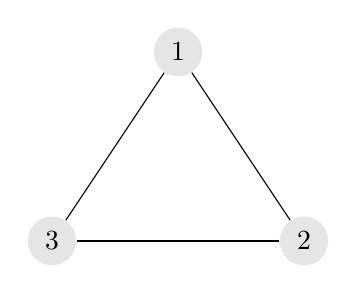
\begin{tikzpicture}
  [scale=.8,auto=left,every node/.style={circle,fill=gray!20}]
  \node (n1) at (5,5) {1};
  \node (n2) at (7,2)  {2};
  \node (n3) at (3,2)  {3};

  \foreach \from/\to in {n1/n2,n1/n3,n2/n3}
    \draw (\from) -- (\to);
\end{tikzpicture}
\caption{A network of three peers}
\label{fig:threepeers}
\end{figure}


\subparagraph{Firewall Problems}
In a test having one process running on a server in Internet and outside of the local network and having two
different processes running on one laptop but on different ports it is observed that the changes (sets) in the
Internet does not replicate to the local processes but the changes from local processes are being replicated to the other process.

\subparagraph{Conclusion}
Having a network between local and Internet processes in the above mentioned method is not reliable. 
Repeating the tests with only local processes which are bootstrapping to one of them and running the setter/getter
methods showed that even in this scenario it is not reliable and one can not guarantee that the desired value will be returned.

\section{Other Works}
There are a number of other notable works that we did not discuss here but they are worth mentioning.
Moreover this enlarges our vision of state of the art and let us to know more similar efforts 
which we might take advantage of them in future.

\subsection{The Raft Consensus Algorithm}
``Raft\cite{ongaro2014search} is a consensus algorithm that is designed to be easy to understand. ''
``Consensus is a fundamental problem in fault-tolerant distributed systems.
Consensus involves multiple servers agreeing on values. Once they reach a decision on a value, that decision is final.''
\footnote{\url{http://raftconsensus.github.io/}}

\subsection{RADICAL Ensemble MD Toolkit}
As described on their website\footnote{\url{http://radical-cybertools.github.io/ensemble-md/index.html}}:
``The Ensemble MD Toolkit is a Python library for developing and executing large-scale ensemble-based
Molecular Dynamics (MD) simulations and workflows. It is being developed by the RADICAL Research
Group at Rutgers University. Ensemble MD Toolkit is released under the MIT License.''

\subsection{Concoord}
``ConCoord is a novel coordination service that provides replication and synchronization 
support for large-scale distributed systems. ConCoord employs an object-oriented approach, 
in which the system creates and maintains live replicas for Python objects written by the user. 
ConCoord converts these Python objects into Paxos Replicated State Machines (RSM) and enables clients
to do method invocations on them transparently as if they are local objects.''\footnote{\url{https://pypi.python.org/pypi/concoord}}

ConCoord has been used as underlying technology to create OpenReplica\footnote{\url{http://openreplica.org/}}, 
a coordination service for distributed applications.\cite{altinbuken2012commodifying}

\subsection{COSMOS}
``A Python library for workflow
management that allows formal description of pipelines and partition-
ing of jobs. In addition, it includes a user interface for tracking the
progress of jobs, abstraction of the queuing system and fine-grained
control over the workflow.''\cite{Gafni30062014}

\subsection{Weaver}
``Weaver\cite{Bui_weaver:integrating} is a high-level framework that enables the integration of distributed computing abstractions
into scientific and data processing workflows using the Python programming language. 
This takes advantage of users' familiarity with Python, minimizes barriers to adoption, 
and allows for integration with a rich ecosystem of existing software.``\footnote{\url{http://cs.uwec.edu/~buipj/research/software/weaver.html}}

\subsection{iRod}
From iRod's documentation\footnote{\url{http://irods.org/wp-content/uploads/2012/04/iRODS-Overview-November-2014.pdf}}:

iRODS is open-source, data management software that lets users:
\begin{itemize}
\item access, manage, and share data across any type or number of storage
systems located anywhere, while maintaining redundancy and security,
and
\item exercise precise control over their data with extensible rules that
ensure the data is archived, described, and replicated in accordance
with their needs and schedule
\end{itemize}

\subsection{Ceph}
``Ceph is a distributed object store and file system designed to provide excellent performance, 
reliability and scalability\footnote{\url{http://ceph.com}}."


\iffalse
\subsection{Concoord}
Describe why it is not suitable for us. It allows single object sharing.

\section{Distributed Workflows}
For our last section of this chapter we also need to define some parameters in the beginning:
\begin{itemize}
\item Deployment complexity
\item Data provision methods
\item State preservation
\item Centralization
\item Required user rights
\item Runtime control
\item Applicability
\end{itemize}

In this section we introduce a number of existing scientific workflow systems.
\subsection{COSMOS}\cite{Gafni30062014}
\subsection{Weaver}\cite{Bui_weaver:integrating}
\fi
